Mongodb is a schemaless document oriented database developed by MongoDB Inc.( then 10gen Inc.) and Open Source Community. It is intended to be flexible data model, fast and Multi-datacenter scalable system written in C++.
\subsubsection{Data Model}
MongoDB uses the concept of \textit{collections} and \textit{documents} to model data. Collection contain any type of documents but generally it has documents with  similar schema. Data has flexible schema where collections do not enforce document to structure rather requirements of our application. A collection is analogous to table of relational database or collection of XML database. Documents are modeled as a data structure following the JSON format which actually store as BSON~\cite{bson}, a binary variant of JSON.  In Mongodb, there are two principle that allow application to represent documents and their relationship: \textit{reference} and \textit{embedded documents}. 
\todo{ need to change following image/json according to xmark data}

\paragraph{Reference}
Reference stores the relationships between data by including links and references from one document to another as in  Figure~\ref{fig:mongodb-ref-doc}. The application can resolve these reference to access the related data\todo{Mongodb data model pg4}
\paragraph{Embedded}
Embedded documents captures relationships between the data by storing related data in a single document structure. The documents in this method are structured as sub-documents\todo{...??} in the in the form of Array or/and Object~\cite{nosql/comparision}. 
\label{mong-xmark-indexing}

\paragraph{Indexing} 
Each document in Mongodb is uniquely identified by a field \textit{\_id} which is a primary index. Hence the collection is sorted by \textit{\_id} by default~\cite{nosql/comparision}.
In addition to primary index, Mongodb supports various user defined indexes for field values of documents including single field index, multikey index, multidimensional index, geo-spatial index, text index and hash index.  Single field, multidimensional and multikey index are organized using B-tree whereas geospatial index is implemented using quad trees.

To index a field that contains a array value, MongoDB provides special indexing called "Multikey". These \textit{multikey} indexes allow MongoDB to return documents from queries using the value of array. 
\begin{figure}
	\centering
	\subfigure[Reference document]{
		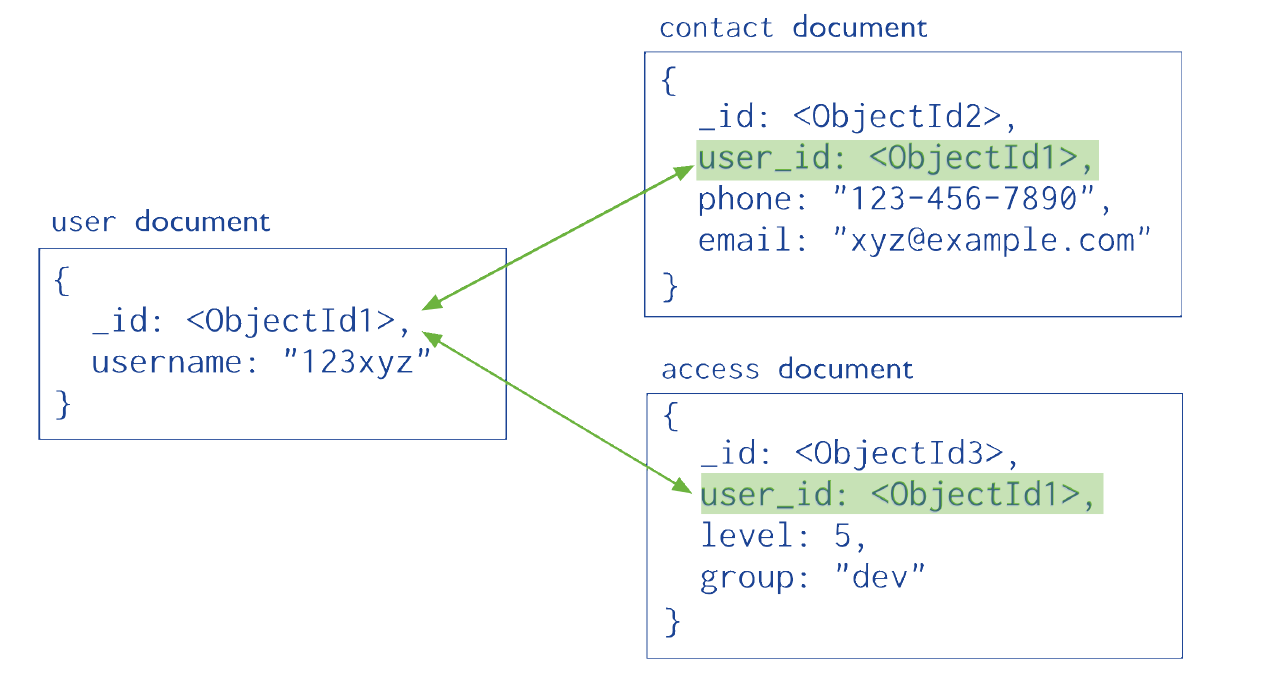
\includegraphics[width=0.44\textwidth]{img/mongodb-reference}
		%\caption{R-tree structure}
		\label{fig:mongodb-ref-doc}
	}
	\centering
	\subfigure[Embedded document]{
		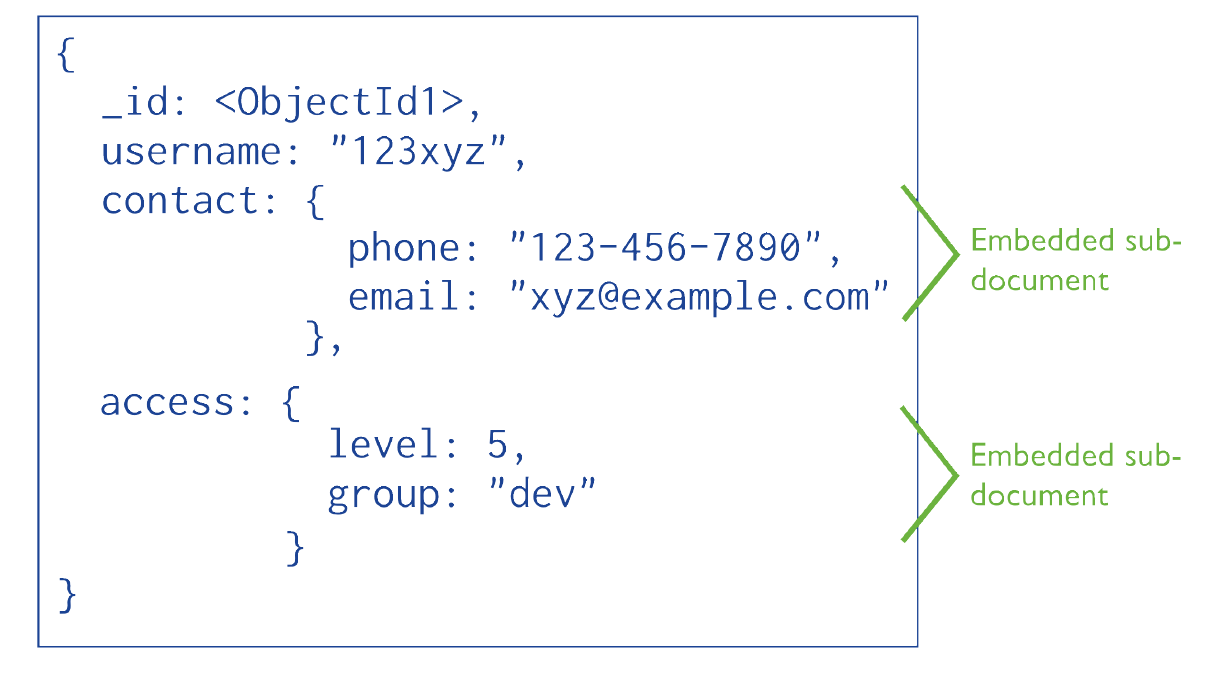
\includegraphics[width=0.44\textwidth]{img/mongodb-embedded}
		%\caption{R-tree}
		\label{fig:mongodb-emb-doc}
	}
	\caption{Mongodb document structure}
	\label{fig:mongodb-doc}
	
\end{figure}

\subsubsection{Query Model}
Queries in MongoDB are expressed in a JSON like syntax and send to MongoDB as BSON objects by database drivers\cite{orend2010analysis}. MongoDB's query can be implemented over all documents inside collections, including embedded object and arrays. 
The Query model support following features:
\begin{enumerate}
	\item Queries over documents, embedded subdocuments and arrays
	\item Comparison operators
	\item Conditional Operators
	\item Logical Operators: AND and OR
	\item Sorting 
	\item Group by 
	\item Aggregation per query
\end{enumerate}
In addition to this MongoDB provide a features to for complex aggregation with the use Of MapReduce. The result of MapReduce either can be store as a collection or be removed after result has been return to client\cite{orend2010analysis}.